\section*{Week 41}\label{week41}
\subsection*{What Happend This Week}
This week we have started brainstorming on the \ac{GUI} for the application and
made some considerations as to what will be shown. On \autoref{fig:sketch} a
sketch is shown for our \ac{GUI}, currently the idea is to show where the person is
located on the political spectrum based on its Twitter profile. We have also
considered showing where the user stands compared to the user's friends. Aside
from that, we made some smaller edits to the report.

\begin{figure}[H] 
	\centering 
	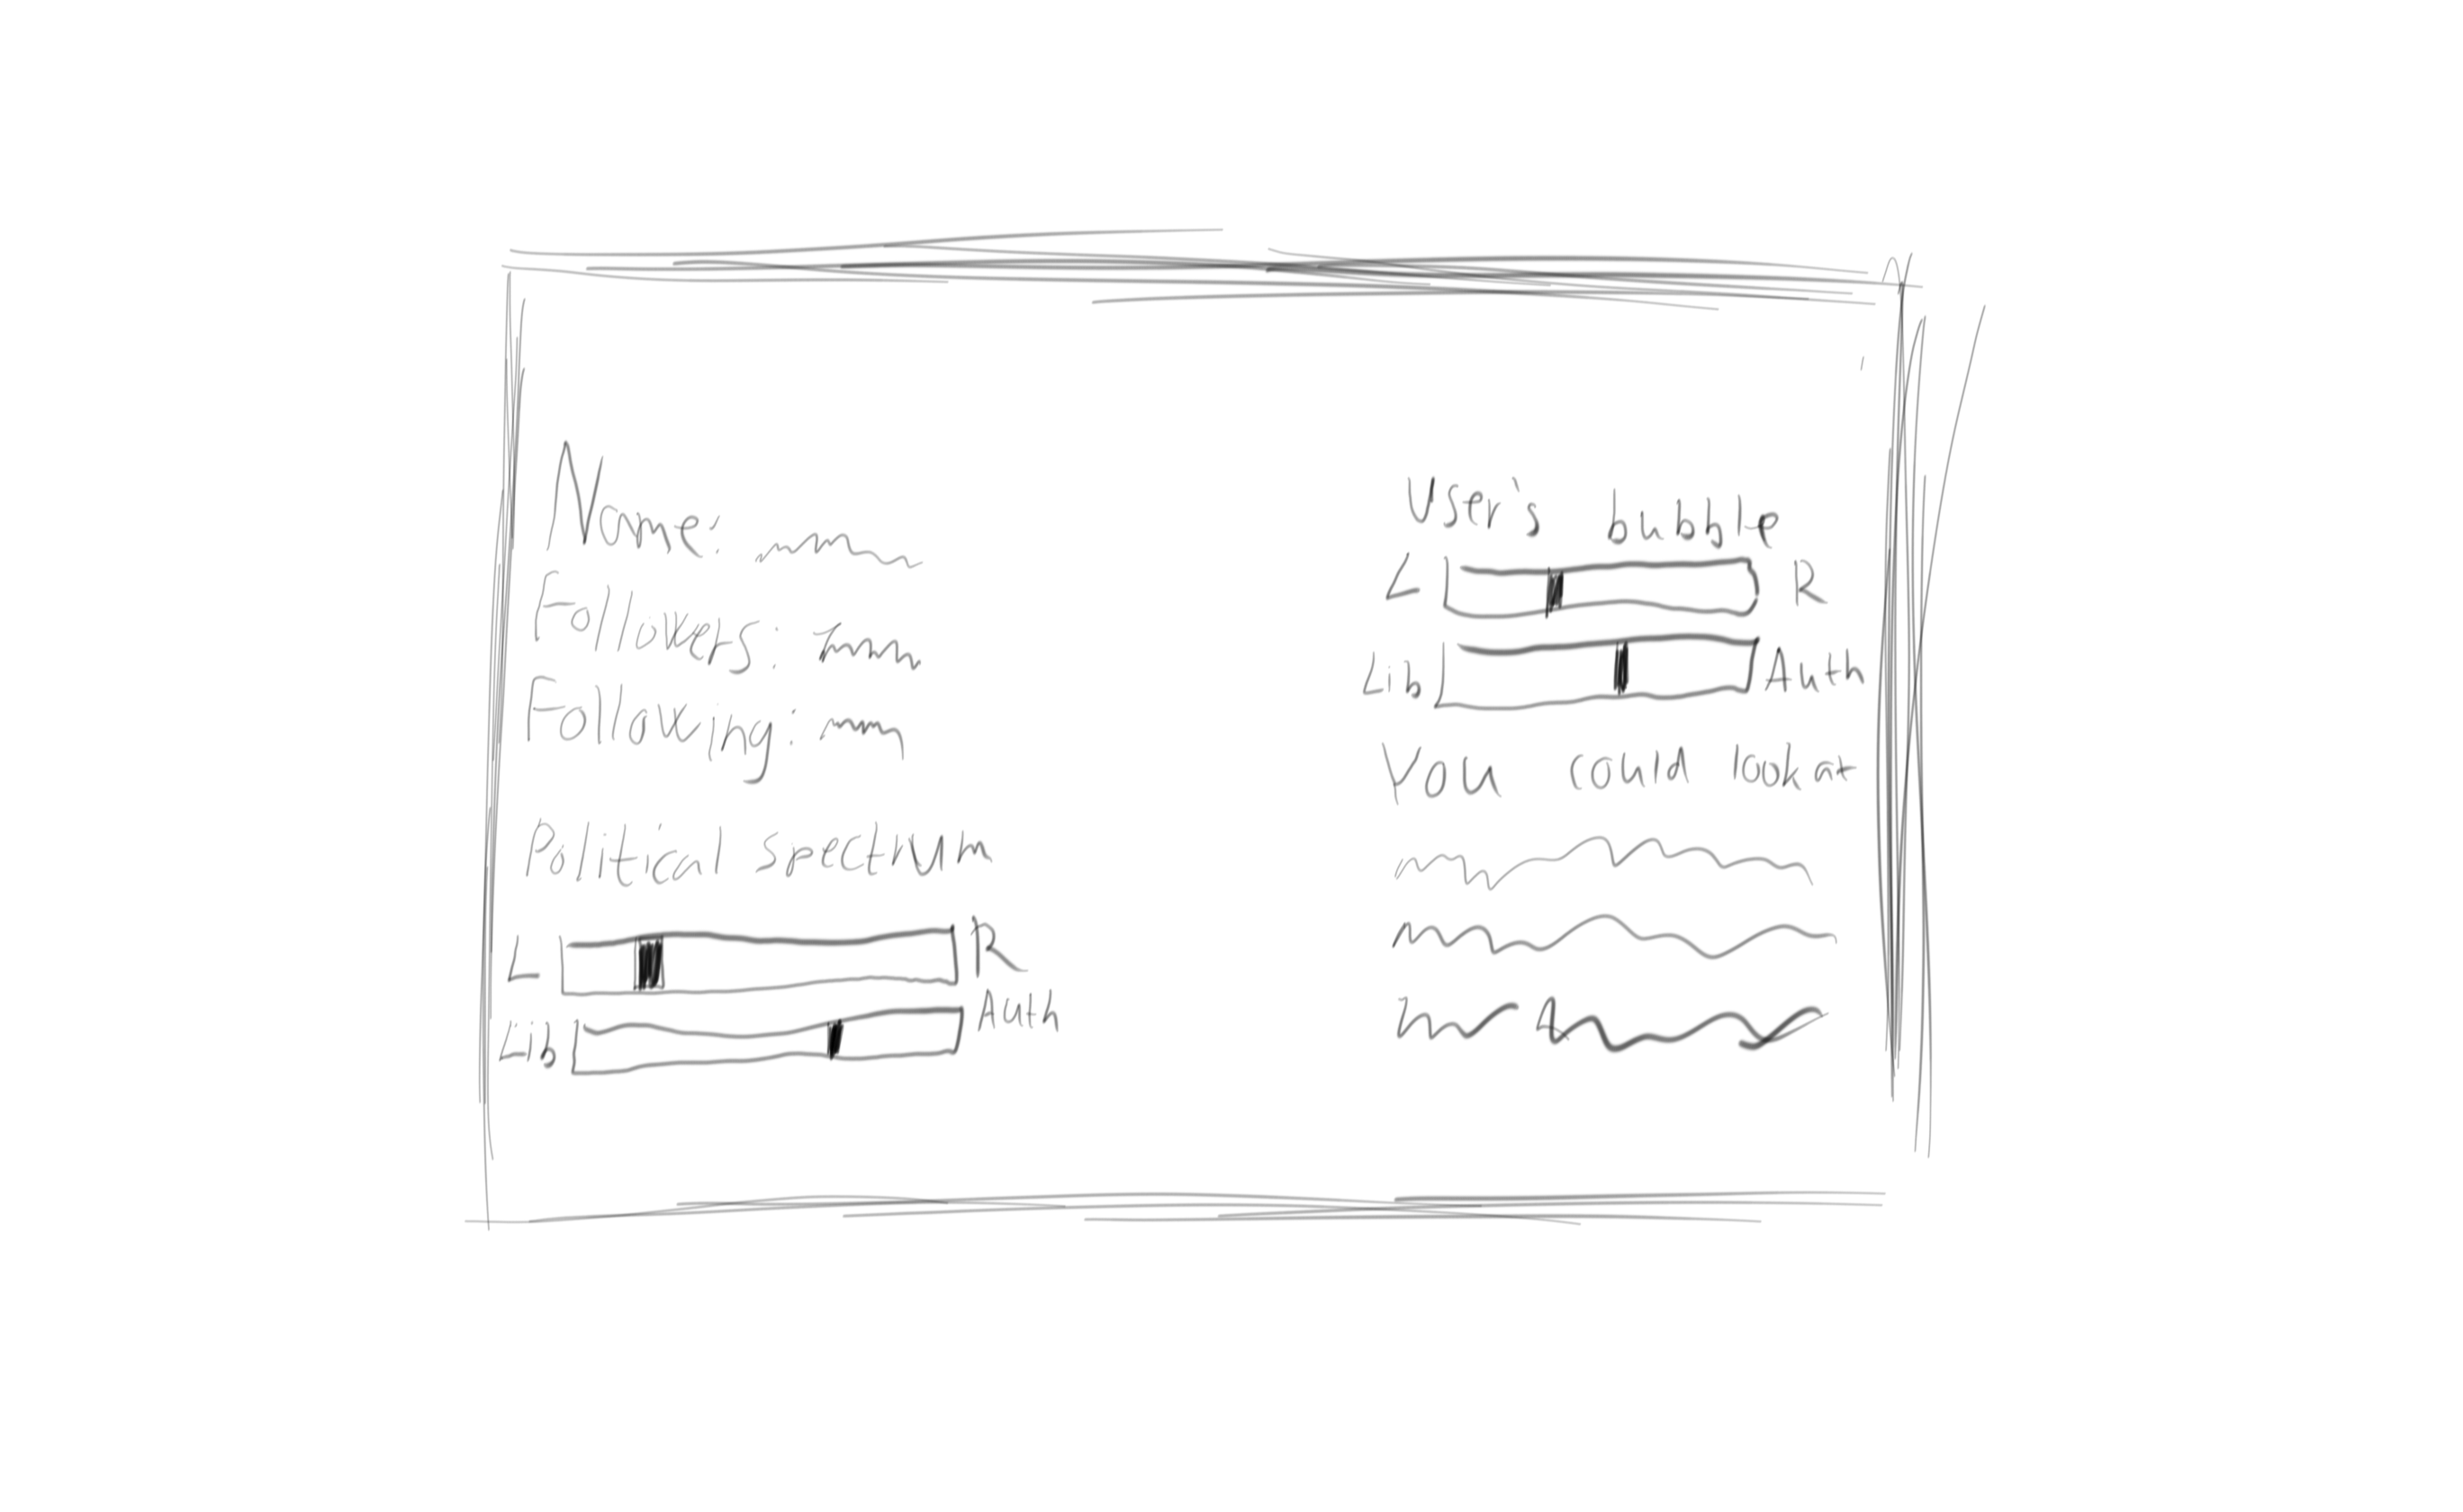
\includegraphics[width = 0.7\textwidth]{figures/guisketch2.png}
	\caption{A sketch of our initial idea for a \ac{GUI}.}
	\label{fig:sketch}
\end{figure}

\subsection*{Reflection} 
During the development of the \ac{GUI}, we found that
we had not given much thought to what we wanted to present the user of the
application with. While designing the \ac{GUI} we came up with other cool
features we could extrapolate from the gathered data, such as information on the
user's friends, it could have been useful to do this a little earlier. Our
supervisor informed us that we did not need to bring much from courses, and our
ideas were fitting, although there were no issues, this should have been ensured
earlier. Our research chapter needed to be restructured a little to be more
coherent.


\subsection*{Next Week}
We will finish the restructuring of the report and continue development of the
program, and get started on developing the front end.



% Worked on a GUI section (DEB terms), specifically we drew a storyboard and a
% sketch of the gui.
% 
% Reworked text and fixed grammatical errors. Reworked the title in analysis,
% began on problem statement, and finished working on most of the analysis.
% 
% Fixed the threads of the program We are now able to find the average political
% value of a bias.
% 
% Scheme delivery